{\documentclass[authoryear]{elsarticle}

\setlength\arraycolsep{2pt}
\setlength{\parskip}{1ex plus 0.5ex minus 0.2ex}
\usepackage{graphicx}
\usepackage{amsfonts}
\usepackage{multirow}
\usepackage{comment}

%\usepackage{chicago}
\bibliographystyle{chicago}



\newcommand{\eps}{\epsilon}
\newcommand{\var}{{\rm var}}
\newcommand{\cov}{{\rm cov}}
\newcommand{\nid}{{\rm NID}}
\newcommand{\diag}{{\rm diag}}
\newcommand{\E}{{\mathrm E}}
\newcommand{\R}{{\mathrm R}}
\newcommand{\RD}{{\tilde{\mathrm R}}}
\newcommand{\Q}{{\mathrm Q}}
\newcommand{\U}{{\mathrm U}}
\newcommand{\Ex}{{\cal E}}
\newcommand{\cor}{\mathrm{cor}}
\newcommand{\tr}{\mathrm{tr}}
\newcommand{\e}{\mathrm{e}}
\newcommand{\de}{\mathrm{d}}
\newcommand{\p}{\mathrm{P}}
\newcommand{\Ln}{\mathrm{Ln}}
\newcommand{\ra}{\varrho}

\newcommand{\minn}{\mathrm{min}_n}
\newcommand{\maxn}{\mathrm{max}_n}
\newcommand{\cq}{\ ,\qquad}


\newcommand{\ppo}[1]{|{#1}|^+}

\newcommand{\ssection}[1]{%
  \section[#1]{\textbf{\uppercase{#1}}}}
\newcommand{\ssubsection}[1]{%
  \subsection[#1]{\normalfont\textbf{#1}}}


%\renewcommand{\labelenumi}{(\roman{enumi})}

\newcommand{\eref}[1]{(\ref{#1})}
\newcommand{\fref}[1]{Figure \ref{#1}}
\newcommand{\sref}[1]{\S\ref{#1}}
\newcommand{\tref}[1]{Table \ref{#1}}
\newcommand{\aref}[1]{\ref{#1}}

\title{The tradeoff insurance premium based on conditional percentile rank deviations}
\author[acst]{Weihao Choo\corref{cor1}}
\author[acst]{Piet de Jong}
\ead{weihao.choo@mq.edu.au}

\cortext[cor1]{Corresponding author}
\address[acst]{Department of Actuarial Studies Macquarie
University, NSW 2109, Australia.}



\begin{document}

\begin{abstract}
The tradeoff premium extends existing ``one-sided'' premium principles and risk measures to address both overpricing and underpricing concerns. The tradeoff premium is a weighted average loss, where weights increase with ``conditional percentile rank deviations'' from a reference point. Tradeoff premiums reduce to loss aversion reserves or equivalently distortion risk measures when only underpricing concerns are present. Tradeoff premiums are also expected losses under a modified probability distribution based on cumulative prospect theory.
\end{abstract}

\begin{keyword}
Two-sided premium, weighted premium, overpricing, underpricing, distortion risk measure
\end{keyword}


\maketitle

\section{Introduction and overview}

This paper proposes the ``tradeoff premium.'' The tradeoff premium is a weighted average loss from an insurance contract. The weights in the average increase as losses move into both the upper and lower tail.
, reflecting aversion to both under and overpricing . Overpricing causes loss of business in a competitive market and underpricing depletes capital. The tradeoff premium is  ``two-sided'' and contrasts with  existing ``one sided''  premiums focussing solely on  ``large'' loss outcomes and underpricing. The tradeoff premium is shown to comprise of the average loss, a loading to avoid underpricing and a discount to avoid overpricing.  Avoiding both over and underpricing involves a tradeoff, and relative sizes of the loading and discount determine the overall magnitude of the tradeoff premium.

The tradeoff premium depends on a ``reference point'' dividing over and underpricing. Changing the reference point shifts the relative aversion between over and underpricing. For example increasing the reference point decreases the tradeoff premium by raising the relative aversion to overpricing. A zero reference point implies nil aversion to overpricing, and yields the usual``one-sided'' premiums.

Weights in the tradeoff premium are determined by an aversion function on the ``departure" between loss outcomes and the reference point. The departure is measured using ``conditional percentile rank deviation''. Conditional percentile rank deviations are differences between percentile ranks of loss outcomes and the reference point,  scaled to fit the unit interval. Using this weight formulation, the tradeoff premium is the average loss under a density transformed using cumulative prospect theory, where cumulative probabilities of moderate and extreme outcomes are weighted less and more, respectively. If the reference point is zero, the tradeoff premium reduces to distortion and spectral risk measures.

Tradeoff premiums are two-sided versions of existing one-sided premiums or risk measures, again emphasizing concerns to reflect both extremes of the loss distribution. For instance the ``two-sided Value-at-Risk'' is a weighted average of upper and lower extreme percentiles. The ``two-sided Conditional-Tail-Expectation'' is also a weighted average, of conditional expected losses in the upper and lower tails. In both examples, changing the reference point shifts the relative representation of ``large'' and ``small'' losses in the tradeoff premium.

Other properties of the tradeoff premium are explored. The tradeoff premium is ``nearly coherent.''  Only the subadditivity property of coherence is not satisfied since both the loading and discount in the tradeoff premium reduce when insurance contracts are aggregated, to reflect lower loss variability from diversification. The overall impact of aggregation hence involves a tradeoff.

Finally the tradeoff premium is ``balanced'' when it is equal to the selected reference point. If this occurs, conditional percentile rank deviations are linked to actual premium surplus or shortfall. The ``balanced premium'' always exists and is unique. In addition it equalises expected premium shortfall and surplus under a transformed loss density, hence balancing conflicting objectives to avoid over and underpricing.

Remaining sections are as follows. Section \aref{definition} defines and justifies the tradeoff premium for a random loss using a specified reference point and aversion function. Section \aref{prospecttheory} expresses the tradeoff premium as an expected loss under a modified probability distribution consistent with cumulative prospect theory. Section \aref{negativerelationship} shows the tradeoff premium decreases with the reference point due to increasing relative aversion to overpricing, and is equivalent to loss aversion reserves and distortion risk measures for a zero reference point. Section \aref{balancedpremium} defines the balanced premium as a special case when effects of overpricing and underpricing concerns are equalized. Other links with existing literature are discussed in \sref{otherlinks}. Section \aref{premiumloading} decomposes the premium loading into a discount and markup, typical of a profit maximizing firm receiving a separate volume benefit. Theoretical examples of tradeoff premiums are shown in \sref{theoreticaleg}. Section \aref{policyholderperspective} shows the tradeoff premium is applicable to a policyholder trading off financial consequences of large loss outcomes and the ``wastage'' of insurance coverage when loss outcomes are favourable. Practical properties of tradeoff premiums are discussed in \sref{properties}. Finally \sref{numericaleg} calculates tradeoff and balanced premiums assuming a gamma loss distribution and power aversion function.


\section{The tradeoff premium}\label{definition}

The tradeoff premium is a weighted average loss. Weights are determined by the aversion to pricing errors based on departures of loss outcomes from a reference point. Negative and positive departures respectively indicate overpricing and underpricing.

Consider an insurance loss $x\geq 0$ with distribution function $F$ and percentile rank $u\equiv F(x)$.  Then $u$ is uniformly distributed on the unit interval. Given a reference percentile rank $0\le\pi\le 1$ define the percentile pricing error  as\footnote {Throughout this paper the notation eg. $(u<\pi)$ indicates the indicator of $u<\pi$.   That is $(u<\pi)$ is 1 or 0 according to whether $u<\pi$ or otherwise.}
\begin{equation}\label{distance}
\delta_\pi(u) \equiv  (u\leq\pi)\frac{\pi-u}{\pi}+(u>\pi)\frac{u-\pi}{1-\pi} \;.
\end{equation}
The percentile pricing error function $\delta_\pi$ is combined with an aversion function $\phi\ge0$ to define the percentile pricing error aversion function $\phi_\pi\equiv \phi\circ \delta_\pi$ and the tradeoff premium
\begin{equation}\label{tradeoff}
r_\pi\equiv\E\{x\phi_\pi(u)\} = \mu +\sigma\sigma_{\phi}\cor\{x,\phi_\pi(u)\}\,
\end{equation}
where $\E$ calculates expectations under $F$. The second relation follows, as shown below, from assuming $\E\{\phi(u)\}=1$, and the fact that $\phi_\pi(u)$ has standard deviation equal to that of $\phi(u)$, denoted $\sigma_\phi$.   Further $\mu$ and $\sigma$ denote the mean and standard deviation of $x$, while $\cor$ denotes correlation.

The tradeoff premium $r_\pi$ in \eref{tradeoff} uses percentile rank $\pi$ to measure the pricing error $\delta_\pi(u)$ for various loss percentile ranks $u$. The pricing error $\delta_\pi(u)$  is evaluated with aversion function $\phi$ and the resulting values are used to weigh, together with probabilities, loss outcomes to calculate the tradeoff premium.   The tradeoff premium is equivalent  to the mean  $\mu$ of the loss plus the multiple $\sigma_\phi\cor\{x,\phi_\pi(u)\}$ of the loss standard deviation $\sigma$.  The correlation $\cor\{x,\phi_\pi(u)\}$ is the only term in \eref{tradeoff} depending on $\pi$, in addition to $\phi$ and $F$.

The left panel in \fref{pricingerrorgraph} displays $\delta_\pi(u)$ as a function of $0\le u\le 1$ for various $\pi$. The right panel displays $\phi_\pi(u)=\phi\{\delta_\pi(u)\}$ assuming $\phi(u)=5u^4$ and for the same $\pi$'s as used in the left panel. Note $\delta_\pi(u)$ increases linearly from $0$ to $1$ as $u$ departs from $\pi$. In addition $\phi_\pi(u)$ is an increasing transformation of $\delta_\pi(u)$ using $\phi$. The following subsections consider properties of $\delta_\pi$ and $\phi_\pi$ in further detail.
\begin{figure}
  \begin{center}
    \begin{tabular}{cc}
      \resizebox{60mm}{!}{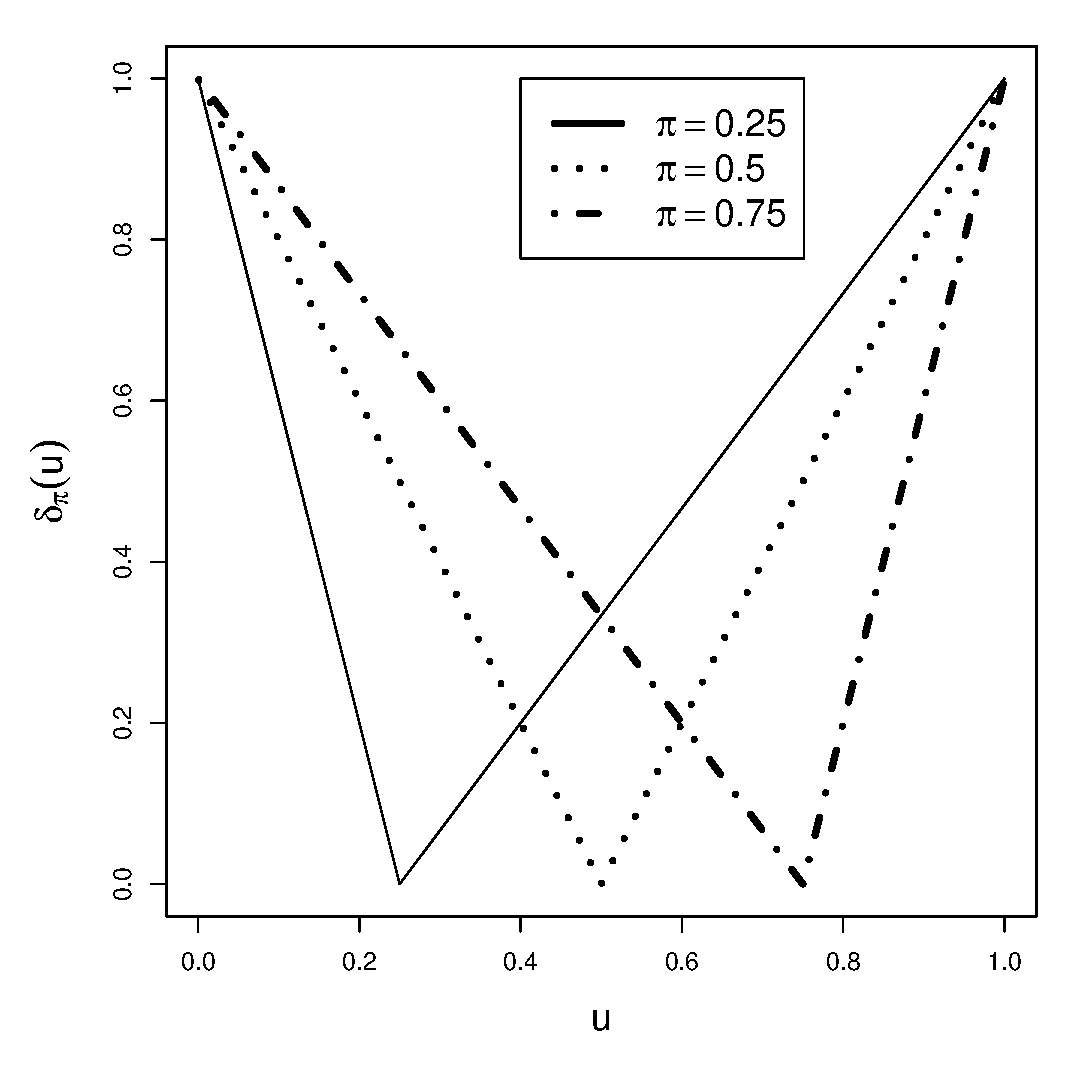
\includegraphics{errorvarypi.eps}}
      \resizebox{60mm}{!}{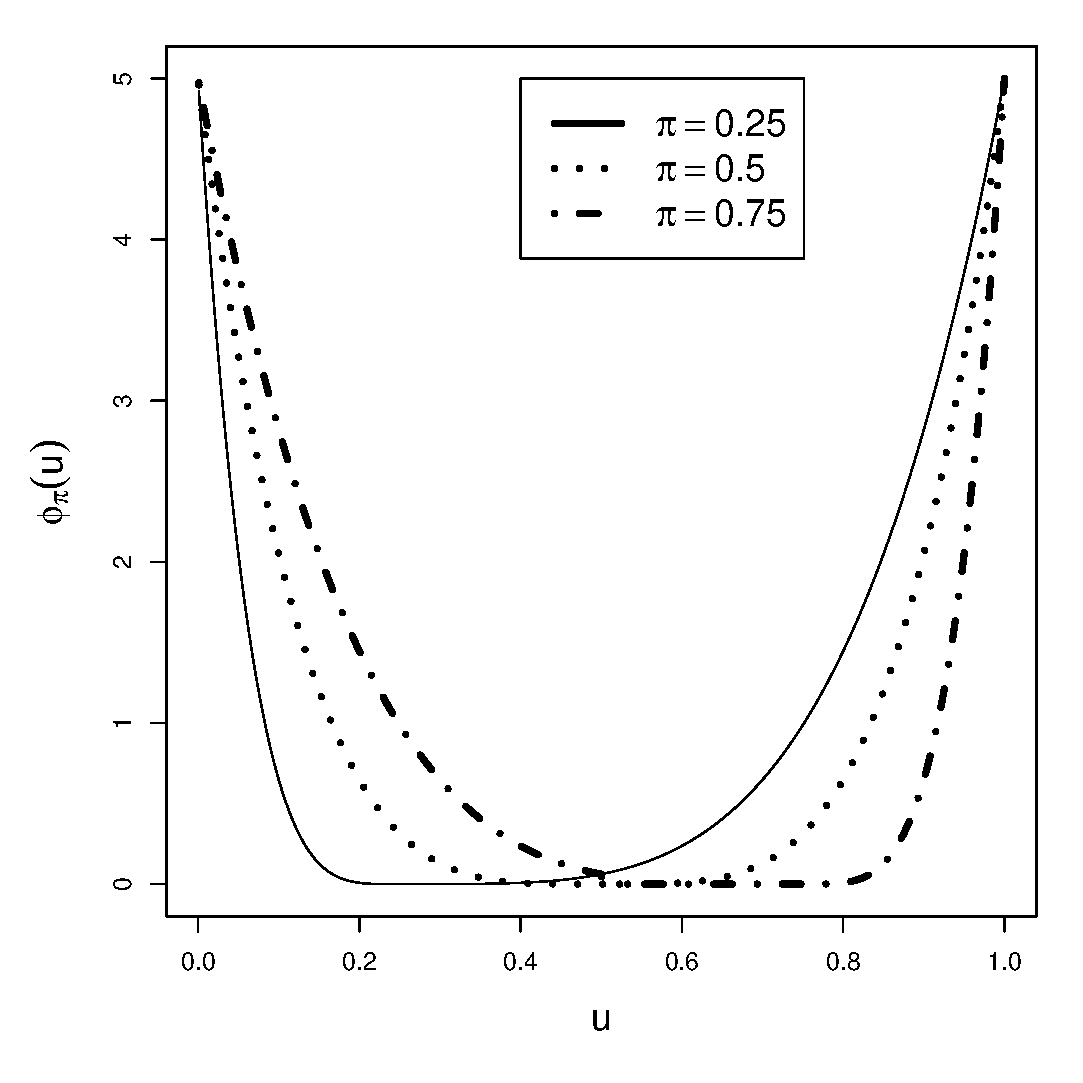
\includegraphics{aversionvarypi.eps}} \\
    \end{tabular}
    \caption{Plots of $\delta_\pi(u)$ (left panel) and $\phi_\pi(u)=\phi\{\delta_\pi(u)\}$ (right panel) against $u$ assuming $\phi(v)=5v^4$ and $\pi=0.25$, $0.5$ and $0.75$. }
    \label{pricingerrorgraph}
  \end{center}
\end{figure}




\subsection{Percentile pricing error}

The percentile pricing error $\delta_\pi(u)$ is the first ingredient in the tradeoff premium, and is uniform given $u<\pi$ and given $u>\pi$. Thus $\delta_\pi(u)$ is uniform over all $u$. Hence overpricing errors, occurring if $u<\pi$, underpricing errors, occurring if $u>\pi$, as well as all pricing errors, are uniformly distributed over the unit interval. Overpricing and underpricing errors are equivalently defined to occur if $x<v_\pi$ and $x>v_\pi$, respectively, where $v_\pi\equiv F^-(\pi)$ is the value-at-risk \citep{mcneil2005qrm}  with $F^-$ being the inverse distribution function and is assumed to exist.

Further $\delta_0(u)=u$ and $\delta_1(u)=1-u$, $\delta_\pi(\pi)=0$ and, for any $0<\pi<1$, $\delta_\pi(0)=1=\delta_\pi(1)$. Pricing error is zero when the loss outcome is equal to the reference point, and one when the loss outcome is at its minimum or maximum.


\subsection{Aversion function}

The second ingredient in the tradeoff premium is an aversion function $\phi$, describing the aversion to different pricing errors. Assume $\phi$ is increasing and integrates to one: $\E\{\phi(u)\}=1$ where $u$ is uniform. The unit expectation implies aversion is measured on a relative scale, and consists of both magnification: $\phi>1$, and diminution: $\phi<1$. Neutrality is implied by $\phi=1$.


\subsection{Percentile pricing error aversion}

Combining $\phi$ with $\delta_\pi$ yields the percentile pricing error aversion function $\phi_\pi=\phi\circ\delta_\pi$, used to generate weights when calculating the tradeoff premium. The distribution of $\phi_\pi(u)=\phi\{\delta_\pi(u)\}$ is independent of $\pi$, and identical to that of $\phi(u)$, noting $\delta_\pi(u)$ and $u$ are uniform. Therefore $\E\{\phi_\pi(u)\}=\E\{\phi(u)\}=1$ indicating an average weight of one in the tradeoff premium, similar to \citet{furman2008weighted} for one sided weighted premiums. Further if $\sigma_\phi$ is the standard deviation of $\phi(u)$ then  $\sigma_\phi$ is also the standard deviation of $\phi_\pi(u)$.

Decompose $\E\{\phi_\pi(u)\}$ into conditional expectations below and above $\pi$:
$$
\E\{\phi_\pi(u)\}=\pi \E\left\{\left.\phi\left(\frac{\pi-u}{\pi}\right)\right|u\le\pi\right\}+(1-\pi)\E\left\{\left.\phi\left(\frac{u-\pi}{1-\pi}\right)\right|u>\pi\right\} \;,
$$
and note both conditional expectations are one.  Hence the total unit weight in the tradeoff premium is split between overpricing and underpricing errors according to their respective occurrence probabilities of $\pi$ and $1-\pi$.

The same aversion applies to overpricing and underpricing errors based on aversion function $\phi$. Take $\phi(u)=nu^{n-1}$ as an example, further discussed in \sref{separation}. Then aversion based expectations of overpricing errors $|v_\pi-x|_+$ and underpricing errors $|x-v_\pi|_+$ both focus on the maximum outcome over $n$ independent copies $x_i$  of $x$, leading to the tradeoff premium
$$
v_\pi - \pi\E\left\{\max_{i=1,\ldots,n} (v_\pi-x_i)|x_i<v_\pi\right\}+(1-\pi)\E\left\{\max_{i=1,\ldots,n}(x_i-v_\pi)|x_i>v_\pi)\right\} \;.
$$
A similar decomposition of the tradeoff premium, where there is a tradeoff between overpricing and underpricing errors, exists for any $\phi$ and is shown and discussed in \sref{separation}.


\subsection{Other examples}

The tradeoff premium when $\phi(v)=nv^{n-1}$ is discussed above. Further examples are as follows. If $\phi=1$ then $\phi_\pi=1$  and $r_\pi=\mu$ for all $\pi$. The insurer is neutral to overpricing and underpricing errors.  Further, for any $\phi$, $r_{1/2}=\mu$ if the loss distribution is symmetric. If  $\phi(u)=(u=\alpha)$, the  Dirac delta function with $0<\alpha<1$, then $r_\pi=\pi v_{(1-\alpha)\pi}+ (1-\pi)v_{1-(1-\alpha)(1-\pi)}$. In this case  $\phi$ is not increasing, but  illustrates a two-sided concern for  small and large losses relative to $v_\pi$, based on value-at-risk. Section \aref{separation} provides further examples.

\begin{comment}
Note required since already highlighted in the EML example? Note $\phi_\pi(0)=\phi(0)$, (no error) and $\phi_\pi(1)=\phi(1)$ (maximum overpricing or underpricing error). The equal assessment of over and underpricing implies errors are relative either to over or underpricing errors. The overall concern of overpricing compared  to underpricing is measured with $\pi$. From \sref{negativerelationship}, increasing $\pi$ decreases the tradeoff premium.  If $\pi=1/2$  overpricing and underpricing relative to the median is of equal concern.
\end{comment}




\subsection{Equilibrium pricing}

If  $F(r_\pi)=\pi$,  then the tradeoff premium $r_\pi$ has percentile rank  equal to the reference point $\pi$ used to compute the tradeoff premium. In addition $r_\pi= v_\pi$ hence pricing errors $x-v_\pi$ and premium deviations $x-r_\pi$ are equal. This equilibrium $\pi$ is denoted $\pi_*$ with associated ``equilibrium premium" $r_* = r_{\pi_*}$.

If $\pi\ne\pi_*$, indicating disequilibrium, then $\pi_1=F(r_\pi)$ defines the new reference point yielding an updated tradeoff premium $r_{\pi_1}$.   If $r_{\pi_1}\ne v_{\pi_1}=F^-(\pi_1)=r_\pi$ this iterative step is repeated  to yield $\pi_2$ and $r_{\pi_2}$, and so on.  The elements of the resulting sequence $\pi, \pi_1,\pi_2, \dots$ lie between 0 and 1 and assume there is an accumulation point $\pi_*$ such that $v_{\pi_*}=r_{\pi_*}=r_*$, yielding the equilibrium premium.  Equilibrium premiums are further discussed in \sref{equilibriumpremium}.



\subsection{The standardized tradeoff premium}

The standardized tradeoff premium is
\begin{equation}\label{tradeoff1}
r^*_\pi\equiv \frac{r_\pi-\mu}{\sigma} = \sigma_\phi\cor\{x,\phi_\pi(u)\}\ .
\end{equation}
The right hand side of \eref{tradeoff1} depends on neither $\mu$ nor $\sigma$, implying $r_\pi$ is linear in $x$:    $r_\pi(a+bx)=a+br_\pi(x)$ where $b\geq 0$ and $r_\pi(a+bx)$ and $r_\pi(x)$ are the tradeoff premiums of $a+bx$ and $x$, respectively, using reference point $\pi$. Thus location and scale changes to the loss identically impact the tradeoff premium.

In addition \eref{tradeoff1} expresses $r_\pi$ as a standard deviation premium \citep{young2004premium} using the standard deviation multiple $\sigma_\phi\cor\{x,\phi_\pi(u)\}$. The standard deviation $\sigma_\phi$ measures the overall  aversion to mispricing: large $\sigma_\phi$ implies paranoia to  mispricing while $\sigma_\phi=0$ implies $\phi=1$ and  neutrality to mispricing. In addition the correlation $\cor\{x,\phi_\pi(u)\}$ and hence the tradeoff premium decreases with $\pi$, shown and discussed in \sref{negativerelationship}.


The tradeoff premium trades off overpricing and underpricing concerns, such that $r^*_\pi>0$ implies $r_\pi>\mu$ and the effect of underpricing concerns exceeds that of overpricing concerns. Vice versa when $r^*_\pi<0$. The effects of overpricing and underpricing concerns are explicitly expressed in \sref{separation}.

Also $r^*_{\pi^*}$ is the equilibrium standardized premium.   Given $\phi$ this is an ``absolute" number [not sure what this means].



\subsection{Alternative expressions for the tradeoff premium}

Define the cumulative weight function $\Phi_\pi$ such that $\Phi_\pi'=\phi_\pi$ with $\Phi_\pi(0)=0$.  Then  $\Phi_\pi(1)=1$ and alternative expressions of $r_\pi$ are
\begin{equation}\label{alt}
r_\pi=\int_0^\infty x\phi_\pi\{F(x)\}\de F(x)  = \int_0^1 v_u \phi_\pi(u) \de u
= \int_0^\infty 1-\Phi_\pi\{F(x)\} \de x
\end{equation}
The first expression follows from  \eref{tradeoff}. The second expression substitutes $x=v_u$ and implies values-at-risk are weighted based on the departure of their percentile rank from $\pi$. The final expression uses integration by parts and expresses the tradeoff premium as an expected loss under the modified distribution $\Phi_\pi\circ F$, with density $(\phi_\pi\circ F) \times f$ where $f\equiv F'$ is the original loss density. Hence the likelihood of loss outcomes with percentile rank further from the reference point are magnified, noting $\phi_\pi(u)$ increases as $u$ deviates from $\pi$.

Calculations show
$$
\Phi_\pi(u) \equiv \int_0^u \phi\{\delta_\pi(v)\} \de v = \pi + \frac{(\Phi\circ \delta_\pi)(u)}{\delta_\pi'(u)}
= \pi+\left\{(u>\pi)-\pi\right\}(\Phi\circ \delta_\pi)(u) \;,
$$
where $\Phi=\Phi_0$ is a similar integral of $\phi$. The above expressions follow by noting $\delta_\pi$ is piecewise linear. \fref{CPTlinks} plots $\Phi_\pi(u)$ against $u$ assuming $\phi(u)=nu^{n-1}$, for various $\pi$ and $n$. Note $\Phi_\pi(u)$ is concave for $u\leq \pi$ and convex for $u>\pi$, corresponding to decreasing and increasing $\phi_\pi(u)$, respectively. In addition $\Phi_\pi(\pi)=\pi$ for any  $\phi$.  The right panel in \fref{CPTlinks} shows $\Phi_\pi(u)$, in this example, is nearly constant and equal to $\pi$ for a range of $u$ values around $\pi$. Thus there is a large amount of indifference to, and neglect of, percentile ranks around the reference point. In addition the extent of neglect increases with $n$, since higher $n$ implies greater weight is placed on ``small" and ``large" percentile ranks.

\begin{figure}
  \begin{center}
    \begin{tabular}{cc}
      \resizebox{60mm}{!}{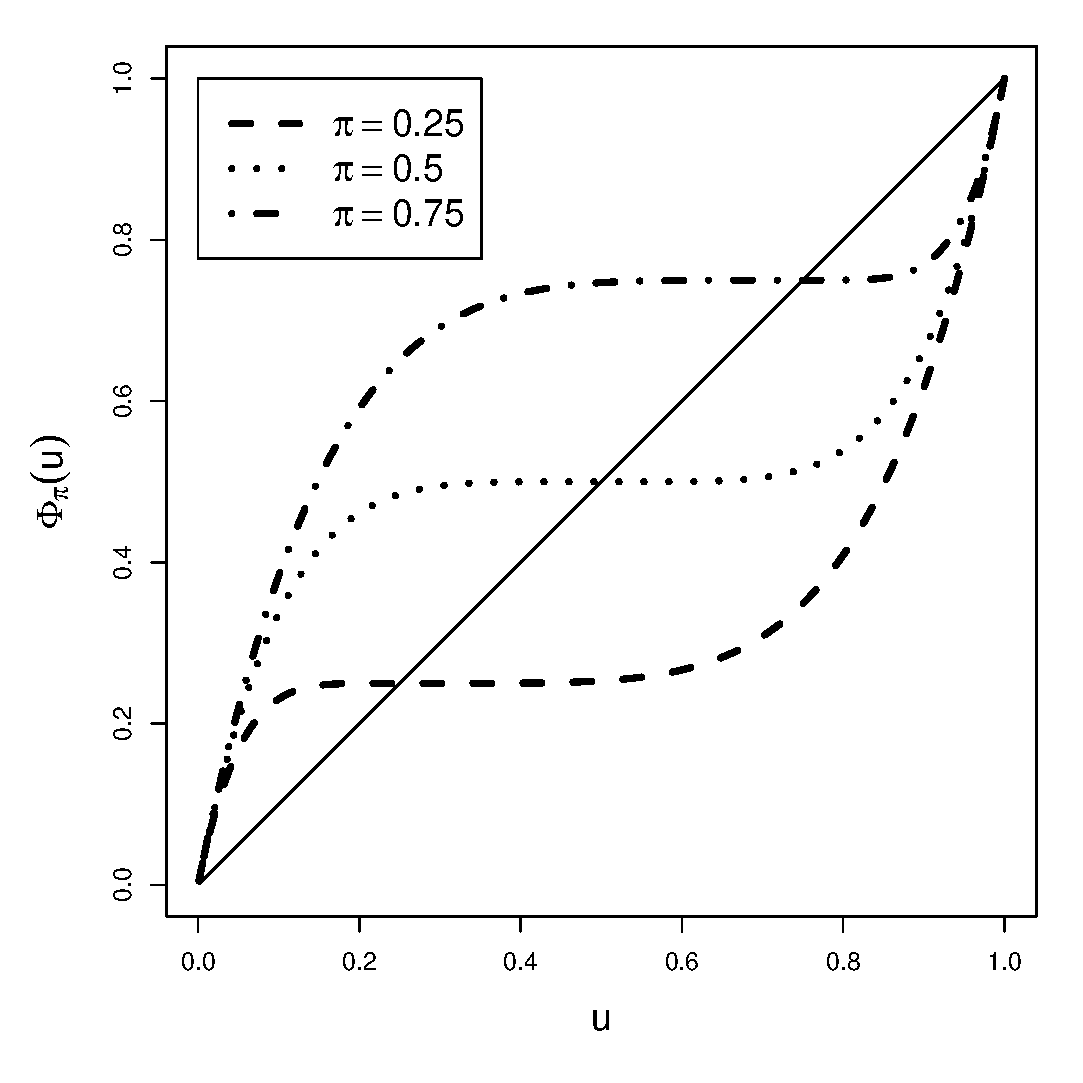
\includegraphics{CPTvarypi.eps}}
      \resizebox{60mm}{!}{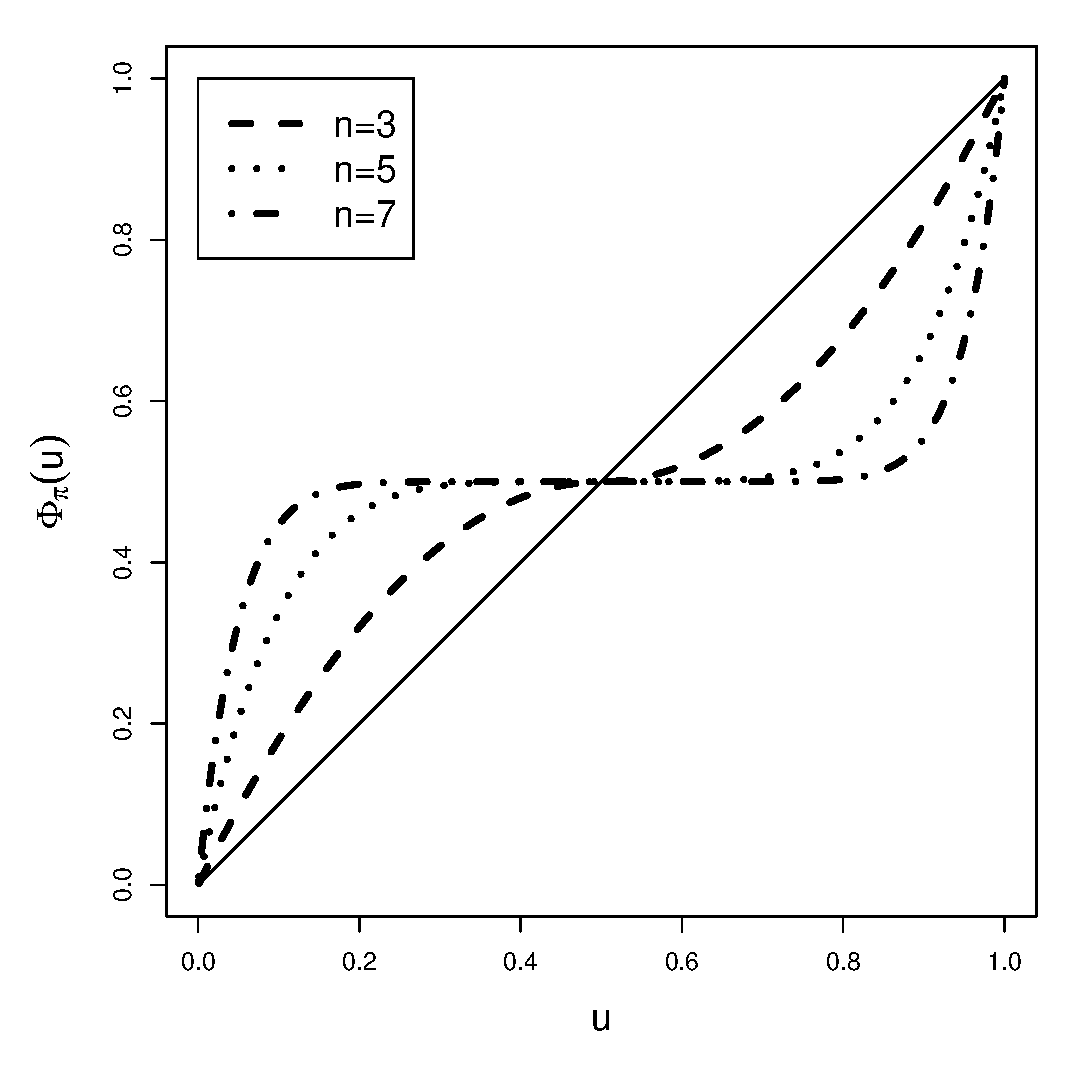
\includegraphics{CPTvaryn.eps}} \\
    \end{tabular}
    \caption{Plots of $\Phi_\pi(u)$ versus $u$ with $\phi(u)=nu^{n-1}$. The left panel assumes $n=5$ and varies $\pi$. The right plot assumes $\pi=0.5$ and varies $n$.}
    \label{CPTlinks}
  \end{center}
\end{figure}

The concavity of $\Phi_\pi(u)$ for $u\leq \pi$ and convexity of $u>\pi$ holds generally, and corresponds to the weight function in cumulative prospect theory or CPT \citep{tversky1992apt}. The weight function transforms cumulative probabilities into decision weights, and is concave and convex for small and large cumulative probabilities, respectively. The weight function derives its shape from the ``principle of diminishing sensitivity" where ``the impact of a given change in probability diminishes with its distance from the boundary." Boundaries are $u=0$ and $u=1$, corresponding to impossibility and certainty in CPT, respectively.






 [Note:  Maybe should look at difference of $\Phi_\pi(u)-\Phi_\pi(v)$ where $u$ and $v$ are ``symmetrically opposed" about $\pi$.   Haven't looked at details but I think the difference will look simple.]


\subsection{Relation to integral operators}

Interpret $\phi_\pi(u)$ in the second integral in \eref{alt} as an integral operator calculating tradeoff premiums at any reference point $0\leq\pi\leq 1$ given values-at-risk at all percentile ranks $0\leq u\leq 1$. The inverse integral operator $\psi_\pi(u)$, assuming it exists, reverses the calculation as
$$
v_u = \int_0^1 r_\pi \psi_\pi(u) \de \pi =  \int_0^1 v_w \int_0^1 \phi_\pi(w) \psi_\pi(u) \de \pi \de w
$$
such  that the inner integral $\int_0^1 \phi_\pi(w) \psi_\pi(u) \de \pi = (w=u)$, or the Dirac delta function.




\begin{comment}

The tradeoff premium equals the expected loss evaluated under a probability distribution modified as in cumulative prospect theory -- CPT \citep{tversky1992apt}.
Possible outcomes are viewed or ``framed"  relative to a  reference point (often the status quo) rather than to the final status. There are different risk attitudes towards gains (i.e. outcomes above the reference point) and losses (i.e. outcomes below the reference point) and there is more aversion to  potential losses than potential gains (loss aversion). Extreme, but unlikely events, are overweighed while ``average" events are underweighed.



Expanding the final term in the above expression yields [Is this expression really necessary/useful?   Also is the material below just repetitive]
$$
\Phi_\pi(u) \equiv (u\leq \pi) \pi \left\{1- \Phi\left(\frac{\pi-u}{\pi}\right)\right\}
+ (u>\pi)\left\{\pi+(1-\pi)\Phi\left(\frac{u-\pi}{1-\pi}\right) \right\} \;,
$$
such that $\Phi_\pi(0)=0$ and $\Phi_\pi(1)=1$. Thus the tradeoff premium is the expected loss under the modified distribution $\Phi_\pi\circ F$ with density $(\phi_\pi\circ F)\times f$ where $f\equiv F'$ is the original density. $\Phi_\pi$ transforms original cumulative probabilities into modified cumulative probabilities, whereas the derivative $\phi_\pi$ weights the density of loss outcomes based on their percentile rank departure from the reference point.
\end{comment}



\section{Varying the reference point and links to distortion risk measures}\label{negativerelationship}

A negative relationship exists between the tradeoff premium and the reference point. In addition the tradeoff premium is bounded by loss aversion reserves
\citep{choo2009loss}, equivalent to distortion risk measures \citep{wang2000cdo}, where only overpricing or underpricing is considered.

Referring to \fref{CPTlinks}, increasing $\pi$ raises $\Phi_\pi(u)$ for all $u$. This result holds for any $\phi$ (see Appendix \aref{proofdominance} for proof) and implies a negative relationship between $r_\pi$ and $\pi$ based on the expression for $r_\pi$ in the right hand side of \eref{alt}. The negative relationship is explained by noting a higher reference point increases the proportion of losses associated with overpricing relative to underpricing, hence decreasing the tradeoff premium.

Since $r_\pi$ is decreasing in $\pi$,
$$
\E\{x\phi(u)\}=  r_0 \ge r_\pi \ge r_1 = \E\{x\phi(1-u)\} \;.
$$
The lower bound  $r_1$ focusses on overpricing with monotonic decreasing weights $\phi(1-u)$, while the upper bound $r_0$ focusses on underpricing with monotonic increasing weights $\phi(u)$. Thus both $r_1$ and $r_0$ are one-sided, whereas $r_\pi$ for $0<\pi<1$ exhibits a two-sided consideration of both overpricing and underpricing. Standardized tradeoff premiums corresponding to $r_1$ and $r_0$ are, respectively
$$
r_1^*= \sigma_\phi\cor\{x,\phi(1-u)\}   \cq r_0^* = \sigma_\phi\cor\{x,\phi(u)\}\ .
$$
Note $r_1$ and $r_0$ fall below and exceed $\mu$, respectively, since $\cor\{x,\phi(1-u)\} \leq 0$ and $\cor\{x,\phi(u)\} \geq 0$. The range of $r_\pi$ is largest and equals that of $x$ when the overall aversion level $\sigma_\phi$ is maximum. Examples are shown in \sref{separation}.

The upper bound $r_0$ is the loss aversion reserve \citep{choo2009loss}. In reserving, aversion increases monotonically with the loss and ``overpricing" is not of concern. The link between $r_0$ and $r_1$ and distortion risk measures \citep{wang2000cdo} is established by substituting $\pi=0$ and $\pi=1$ into the right hand side of \eref{alt}, yielding
$$
r_0 = \int_0^\infty \{1-(\Phi\circ F)(x)\} \de x \cq r_1= \int_0^\infty \{1-(\Phi_1\circ F)(x)\} \de x \;.
$$
Therefore $r_0$ and $r_1$ are distortion risk measures based on distortion operators $\Phi$ and $\Phi_1$, respectively. In addition $\Phi$ is convex, whereas $\Phi_1(v)=1-\Phi(1-v)$ is concave and is known as the dual of $\Phi$ \citep{wang2000cdo}.



\subsection{Interpreting the tradeoff premium as an inverse survival function}

For given $\phi$,  since $r_\pi$  is decreasing in $0\leq\pi\leq 1$, interpret $r_{\pi}$ as the inverse of a survival function:
\begin{equation}\label{interpretation}
r_\pi = (1-F_\phi)^-(\pi) \cq F_\phi(r_\pi)=F_\phi\circ(1-F_\phi)^- = 1-\pi \;,
\end{equation}
where $F_\phi$ is the corresponding distribution function. Note $F_\phi$ is defined from $F$, the distribution function of $x$, and the aversion function $\phi$. In addition $F_\phi$ has the support $[r_1,r_0]$, corresponding to the range of $r_\pi$. The median under $F_\phi$ is $F_\phi^-(1/2)=(1-F_\phi)^-(1/2)=r_{1/2}$, and the mean is
$$
\int_0^1 F_\phi^-(\pi) \de \pi = \int_0^1 r_\pi \de \pi = \E\left\{ x \int_0^1 \phi_\pi(u) \de \pi \right\}
$$
and is the average value of $r_\pi$ over all $\pi$, or a weighted average of $x$ where weights are equal to the mixture $\int_0^1 \phi_\pi(u) \de \pi$ of aversion functions. Section \aref{equilibriumpremium} applies the interpretation \eref{interpretation} when characterizing the equilibrium premium.



\section{The equilibrium premium}\label{equilibriumpremium}


 The equilibrium  premium equalises expected premium surplus and shortfall overlayed with consistent aversion behavior. The equilibrium premium measures the central tendency of the loss distribution, akin to the mean and median.

As mentioned in \sref{definition}, a reference point $\pi$ creates disequilibrium if the associated value-at-risk and tradeoff premium are different: $r_\pi\neq v_\pi$. In disequilibrium, assuming $v_\pi>r_\pi$, aversion $\phi_\pi(u)$ is decreasing for loss outcomes between $r_\pi$ and $v_\pi$, indicating overpricing, even though the tradeoff premium is exceeded implying a premium shortfall. Vice versa when $v_\pi < r_\pi$. The degree of disequilibrium is measured by the difference $r_\pi-v_\pi$, and is expressed by multiplying $x-v_\pi =-|v_\pi-x|_+ +|x-v_\pi|_+ $ by $\phi_\pi(u)$ and taking expectations to yield
\begin{equation}\label{disequilibrium}
r_\pi-v_\pi = - \E\left\{|v_\pi-x|_+\phi_{\pi}(u)\right\} + \E\left\{|x-v_\pi|_+\phi_{\pi}(u)\right\}   \;.
\end{equation}
Since $r_0-v_0>0$ and $r_1-v_1<0$, and $r_\pi-v_\pi$ is strictly decreasing, there exists a unique $\pi=\pi_*$ attaining equilibrium: $v_{\pi_*}=r_{\pi_*}$. Denote the associated equilibrium premium as $r_*\equiv r_{\pi_*}=v_{\pi_*}$. Equilibrium holds noting losses below $r^*$ simultaneously and consistently represent overpricing (since $x<v_{\pi_*}$) and a premium surplus (since $x<r_{\pi_*}$), and vice versa for loss outcomes above $r^*$.

Substituting $\pi=\pi_*$ and $r_{\pi_*}=v_{\pi_*}=r_*$ into \eref{equalisation} implies
\begin{equation}\label{equalisation}
 \E\left\{|r_*-x|_+\phi_*(u)\right\}  = \E\left\{|x-r_*|_+\phi_*(u)\right\} \cq \phi_*\equiv \phi_{\pi_*}
\end{equation}
hence the equilibrium premium equalizes expected premium surplus $|r_*-x|_+$ and premium shortfall $|x-r_*|_+$. The aversion adjustment $\phi_*(u)$ increases in both $|r_*-x|_+$ and $|x-r_*|_+$ hence higher premium surplus and shortfall, respectively, are weighted more heavily. The left hand side of \eref{equalisation}, or the aversion adjusted expected premium surplus, is decomposed as
$$
\E\left\{|r_*-x|_+\phi_*(u)\right\}
= \E\left\{|r_*-x|_+\right\} + \cov\left\{|r_*-x|_+,\phi_*(u)\right\} \;,
$$
and exceeds the original expectation $\E\{|r_*-x|_+\}$ due to the positive correlation between $|r_*-x|_+$ and $\phi_*(u)$ for $|r^*-x|_+>0$.  A similar expansion and interpretation applies to the aversion adjusted expected premium shortfall. Hence aversion adjustment increases both expected premium surplus and shortfall.

The equilibrium premium is equal to the mean or median $\mu$ for a symmetric loss distribution. The result follows by noting $|\mu-x|_+$ and $|x-\mu|_+$ are identically distributed and $\phi_{1/2}(u)$ is symmetric about $u=1/2$, corresponding to the median, if the loss distribution is symmetric. Hence $r_*=\mu$ satisfies \eref{equalisation}.

A similar result as \eref{equalisation} holds for any reference point $\pi$ and corresponding tradeoff premium $r_\pi$:
$$
\E\left\{|r_\pi-x|_+\phi_\pi(u)\right\} = \E\left\{|x-r_\pi|_+\phi_\pi(u)\right\} \;,
$$
by applying similar calculations as \eref{disequilibrium}. However aversion behaves inconsistently with premium surplus or shortfall movements in disequilibrium as noted at the start of this section. For example, if $v_\pi > r_\pi$, then $\phi_\pi(u)$ is decreasing in the shortfall $|x-r_\pi|_+$ for $r_\pi<x<v_\pi$. In contrast aversion is increasing in both the premium surplus and shortfall when in equilibrium.



\subsection{Calculating the equilibrium premium}

The equilibrium premium $r_*$ is the intersection point of $v_\pi$ and $r_\pi$ graphed against $\pi$. This calculation is illustration in \sref{numericaleg}. Alternatively calculate $r_*=r_{\pi_*}$ from $\pi_*$ where $\pi_*$ is the fixed point of $F(r_\pi)$ as a function of $\pi$. Suppose $F(r_\pi)$ satisfies conditions underlying Banach's fixed point theorem \citep{banach1922operations}. Then $r_*$ is calculated as
\begin{equation}\label{iteration}
r_* = \lim_{n\rightarrow\infty} r_{\pi_n} , \quad \pi_{n+1} = F \left( r_{\pi_n} \right)  \;.
\end{equation}
The iterative calculation in \eref{iteration} is interpreted as follows. Given a starting reference point $\pi_0$, the tradeoff premium $r_{\pi_0}$ is first computed. Disequilibrium arises if the tradeoff premium and the reference point are misaligned: $v_{\pi_0}\neq r_{\pi_0}$, and results in an updated reference point $\pi_1=F(r_{\pi_0})$ and tradeoff premium $r_{\pi_1}$. The updated reference point and tradeoff premium are compared, with further updating conducted if disequilibrium persists. The iteration continues until the sequence $\pi_0, \pi_1, \pi_2,\ldots$ converges to $\pi_*$ and the equilibrium premium is $r_*=r_{\pi_*}$. An illustration of the iterative calculations is shown in \sref{numericaleg}.


\subsection{Other interpretations of equilibrium premiums}


The equilibrium premium measures the central tendency of the loss distribution with lower and upper tails magnified by aversion. The mean loss $\mu$ equalizes expected surplus and shortfall:
$$
\E\left( |\mu-x|_+ \right) = \E\left( |x-\mu|_+ \right) \;,
$$
akin to the equilibrium premium $r_*$ in \eref{equalisation}, without aversion adjustment. The equilibrium premium differs from the mean loss depending on the relative impact of aversion adjustment on expected surplus and shortfall. As mentioned above, aversion increases with deviations $|r_*-x|_+$ and $|x-r_*|_+$ leading to ``tail magnification" and an increase in expected surplus and shortfall. For a right skewed loss distribution, expected shortfall increases by a relatively greater extent, hence the equilibrium premium exceeds the expected loss. Vice versa. As illustrated in \sref{numericaleg}, increasing right skewness increases the equilibrium premium.

\begin{comment}
Suppose the equilibrium premium is selected to equalize probabilities, instead of expected amounts, of premium surplus and shortfall. Probabilities are calculated after aversion adjustment with reference point equal to the balanced premium. Then the balanced premium $r^*$ and the corresponding reference point $F(r^*)$ is obtained by solving
$$
(\Phi_{F(r^*)} \circ F )(r^*) = 0.5 \quad \Rightarrow \quad r^* = F^-(0.5)
$$
noting the modified distribution function after aversion adjustment at reference point $\pi$ is $\Phi_\pi\circ F$ and $\Phi_\pi(\pi)=\pi$. The balanced premium is hence the median loss using the hypothetical definition. Note the median loss equalizes surplus and shortfall probabilities without aversion adjustment. Hence in this case including an aversion adjustment does not alter the central tendency of the loss distribution.
\end{comment}

An alternative interpretation and hence approximation of $r_*$ follows from \eref{interpretation} where $r_\pi$ is treated as the inverse survival function $(1-F_\phi)^-(\pi)$ applying exceedence probability $\pi$. Then $r_*$ satisfies $F(r_*) = 1-F_\phi(r_*)$ or equivalently $1-F(r_*)=F_\phi(r_*)$ by rewriting the original equilibrium condition $v_{\pi_*}=r_{\pi_*}=r_*$. Therefore $r_*$ is the midpoint of the distributions $F$ and $F_\phi$, equalizing the cumulative probability under one distribution and exceedence probability under the other distribution. Hence approximations of $r_*$ are
$$
\frac{1}{2}\left\{F^-(1/2)+r_{1/2}\right\} \cq \frac{1}{2}\left(\mu+\int_0^1 r_\pi \de \pi\right)
$$
corresponding to the average of medians or means, respectively, noting $r_{1/2}$ and $\int_0^1 r_\pi \de \pi$ are respectively the median and mean under $F_\phi$.



\section{Numerical calculations}\label{numericaleg}

This section calculates tradeoff and equilibrium premiums assuming a gamma loss distribution and power aversion function. Standardized premiums are considered to eliminate location and scale effects. Both tradeoff and equilibrium premiums increase with the right skewness of the loss distribution. In addition a higher aversion level increases the tradeoff premium when effects of underpricing concerns dominate effects of overpricing concerns.

Assume a gamma loss density and power aversion function with parameters $\alpha,\beta>0$ and $n\geq 1$:
$$
f(x) \propto x^{\alpha-1}\exp(-x/\beta) \cq \phi(u)=nu^{n-1} \;,
$$
for $x\geq 0$ and $0\leq u\leq 1$. Increasing the shape parameter $\alpha$ reduces the right skewness of the loss distribution, with $\alpha\rightarrow\infty$ implying normality. In addition $\beta$ is a scale parameter. The power aversion function is related to the expected-maximal-loss reserve \citep{choo2009loss}, further discussed in \sref{separation}, where a higher value of $n$ increases the overall aversion to pricing error.

Assume $\alpha=2$ and $\beta=1$ in the base case. The mean and standard deviation of $x$ are $\mu=\alpha\beta=2$ and $\sigma=\sqrt{\alpha}\beta=\sqrt{2}$, respectively. Further assume $n=5$, hence the overall aversion is $\sigma_\phi=(n-1)/\sqrt{2n-1}=4/3$. Parameter values are subsequently varied to assess their impact on tradeoff and equilibrium premiums.

The top left panel in \fref{illustration} graphs standardized tradeoff premiums $r_\pi^*$ as a function of the reference point $\pi$. As noted in \sref{negativerelationship}, $r_\pi^*$ is decreasing in $\pi$ due to an increasing emphasis on overpricing. Effects of underpricing concerns outweigh effects of overpricing concerns when $r_\pi^*>0$. Note effects of underpricing concerns are dominant in this case, since $r_\pi^*$ exceed $0$ for most of $\pi$ in the unit interval. This is due to the presence of extreme large losses in the right skewed gamma distribution.

The standardized equilibrium premium $r_*^*$ is shown in the same panel as the intersection between $r_\pi^*$ and standardized value-at-risk $v_\pi^*\equiv (v_\pi-\mu)/\sigma$. Note $r_*^*>0$, indicating the equilibrium premium exceeds the mean loss. A right skewed loss distribution leads to an equilibrium premium exceeding the mean loss, discussed in \sref{equilibriumpremium}.

The top right panel in \fref{illustration} displays the original density $f$ and modified density $f_\pi \equiv (\phi_\pi \circ F) \times f$ at $\pi=0.5$. As shown in \sref{definition}, the tradeoff premium is the expected loss under the modified distribution. Note the modified distribution in this case is bimodal, with separate peaks below and above the reference point.

The bottom left panel in \fref{illustration} shows the impact on tradeoff and equilibrium premiums when the right skewness of the loss distribution reduces from increasing $\alpha$. Note aversion based weights $\phi_\pi(u)$ are independent of the loss distribution, and are higher for extreme loss outcomes further from the reference point. Hence reducing right skewness decreases the tradeoff premium due to a moderation of large loss outcomes. Similarly for the equilibrium premium.

The bottom right panel in \fref{illustration} shows the impact of increasing the overall aversion to pricing error, based on increasing $n$. Tradeoff and equilibrium premiums are generally higher when $n$ increases. The reason is increasing $n$ places greater weight on extreme loss outcomes, and increases premiums for a right skewed distribution where large loss outcomes dominate. However, for a relatively high reference point, higher aversion reduces the tradeoff premium as large outcomes are underweighted due to the focus on overpricing.


\begin{figure}
  \begin{center}
    \begin{tabular}{cc}
      \resizebox{60mm}{!}{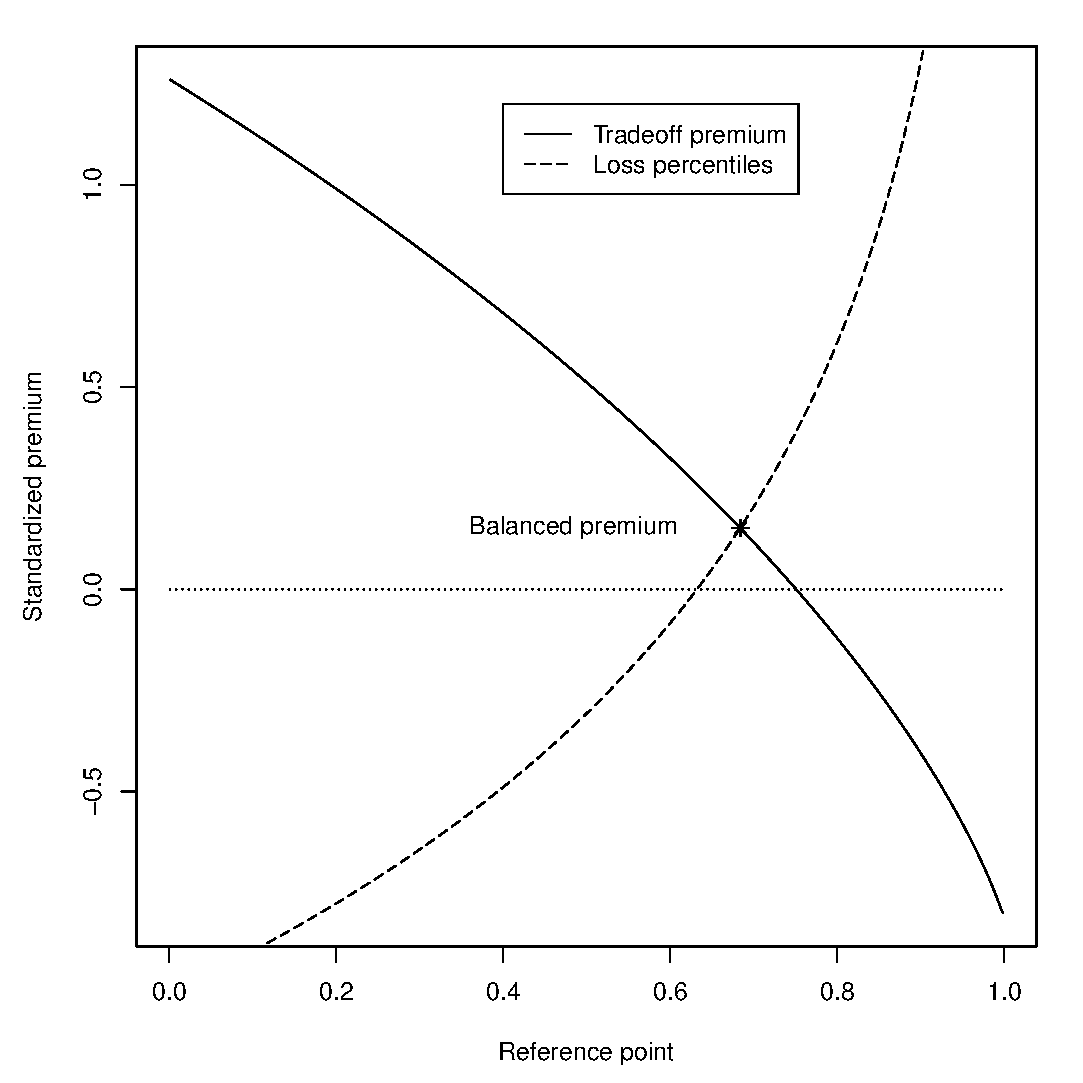
\includegraphics{tradeoffbase.eps}}
      \resizebox{60mm}{!}{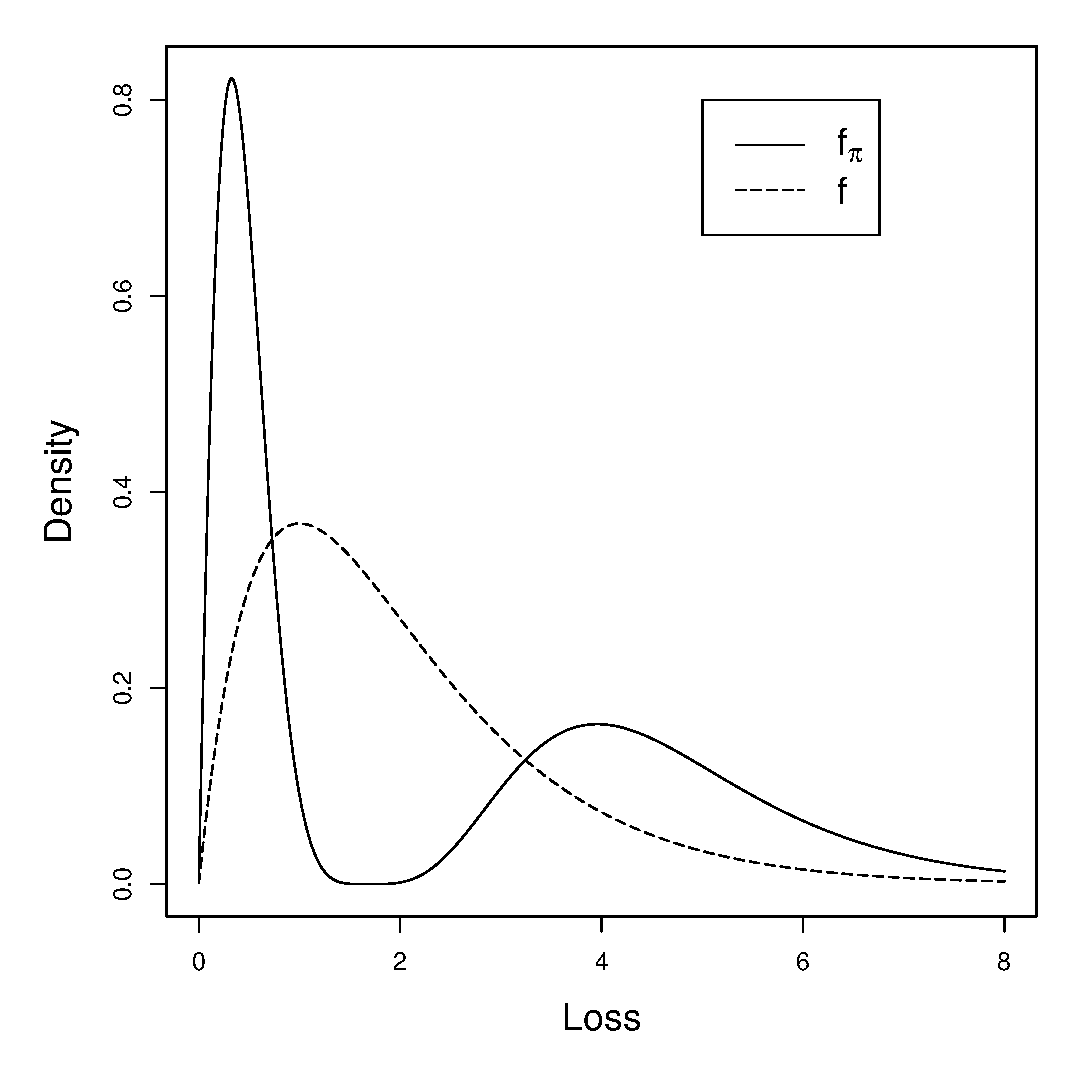
\includegraphics{densities.eps}} \\
      \resizebox{60mm}{!}{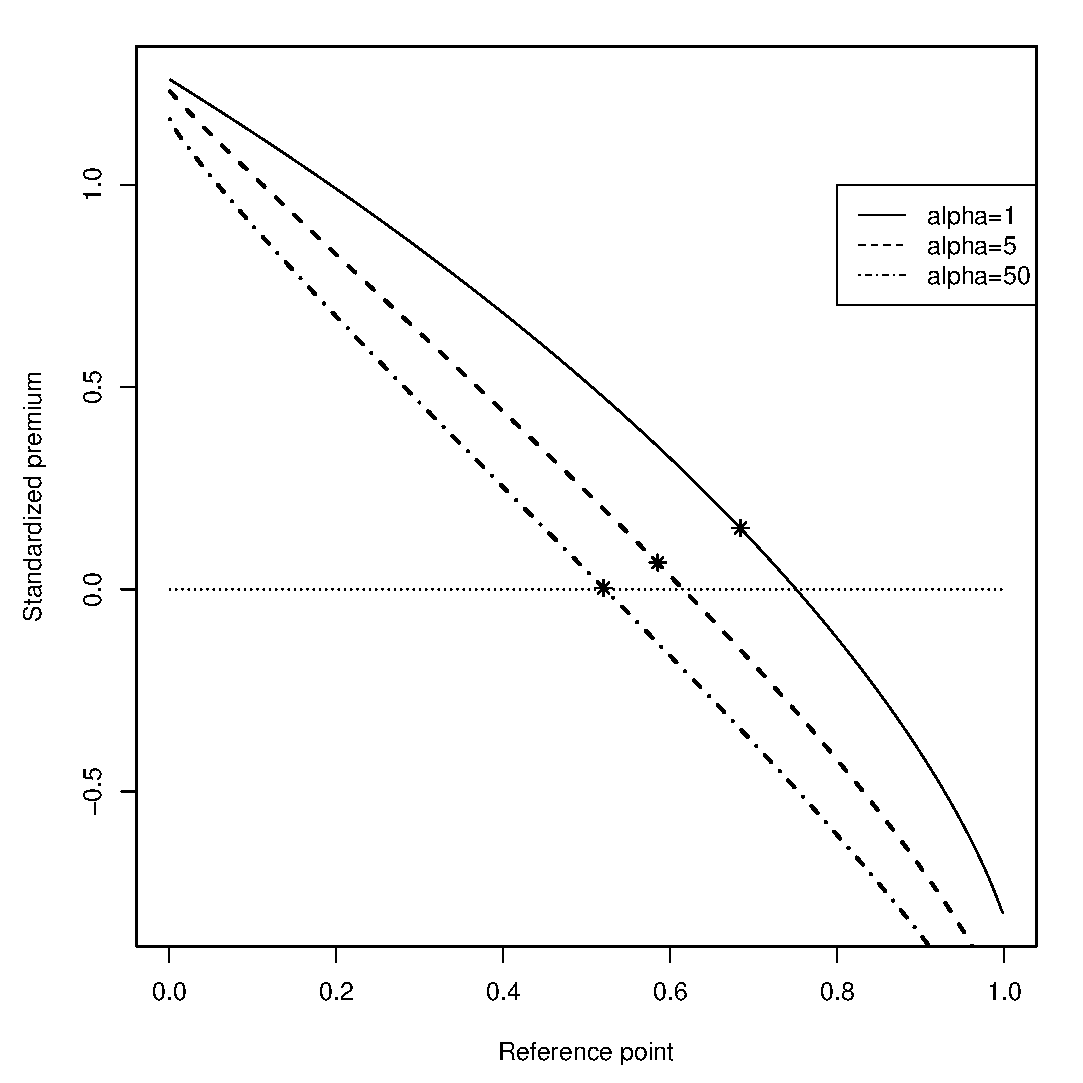
\includegraphics{varyshape.eps}}
      \resizebox{60mm}{!}{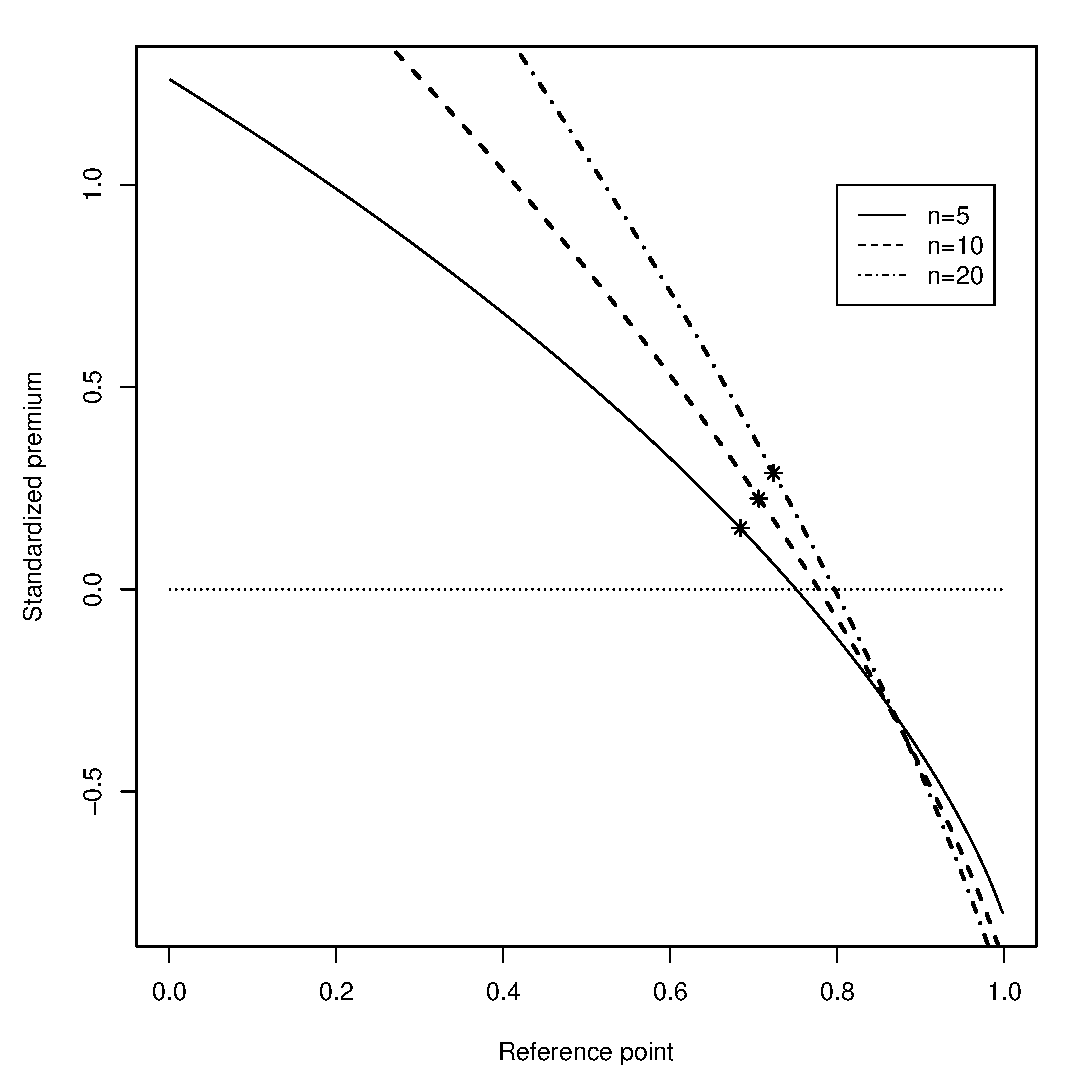
\includegraphics{varyaversion.eps}} \\
    \end{tabular}
    \caption{The top left panel plots $r_\pi^*$ and $v_\pi^*$ against $\pi$. The top right panel plots $f_\pi(x)$ and $f(x)$ against $x$. The bottom left and right panels plot $r_\pi^*$ against $\pi$ for varying $\alpha$ and $n$, respectively. Equilibrium premiums are indicated by asterisks.}
    \label{illustration}
  \end{center}
\end{figure}














\section{Connections to other literature}\label{otherlinks}

The following connects the tradeoff premium to other existing literature, in addition to those discussed in \sref{definition} (standard deviation premium and cumulative prospect theory) and \sref{negativerelationship} (loss aversion reserves and distortion risk measures).

The tradeoff premium is a generalised zero utility premium \citep{heilpern2003rank} by applying rank-dependent utility theory \citep{quiggin1982theory} and assuming a linear utility function. This connection is established by rewriting $r_\pi$ in \eref{tradeoff} as
$$
\E_\pi\left\{U(r_\pi-x)\right\}=0\;,
$$
where $U$ is a linear utility function and $\E_\pi$ calculates expectations with respect to the modified distribution $\Phi_\pi\circ F$. However rank-dependent utility theory assumes $\pi=0$, implying all cumulative probabilities are diminished and underpricing is the only concern. On the other hand the tradeoff premium magnifies only small cumulative probabilities and diminishes large cumulative probabilities allowing for overpricing and underpricing concerns respectively.


\citet{kaluszka2011pricing} applies CPT to the generalised zero utility premium, setting the premium as the reference point. Hence overpricing and underpricing concerns are both taken into account. The equilibrium premium discussed in \sref{equilibriumpremium} is a special case of the tradeoff premium also set equal to the reference point. However \citet{kaluszka2011pricing} does not allow the reference point to vary to reflect differential overpricing relative to underpricing concerns between insurers.




\citet{van2001class} use differential probability adjustment to outcomes above and below a fixed reference point, using two separate distortion operators. The resulting generalized distortion risk measure is applied to asset allocation. However both distortion operators are convex hence cumulative probabilities are consistently diminished, similar to rank dependent utility. In addition \citet{van2001class} expresses the reference point in absolute terms, whereas tradeoff premiums specify the reference point as a percentile rank accommodating all loss scales.





\section{Separating effects of overpricing and underpricing concerns}\label{separation}

The tradeoff premium is decomposed into the value-at-risk at the reference point plus a discount and markup representing overpricing and underpricing concerns, respectively. The discount and markup are distortion risk measures of corresponding pricing errors where larger errors receive greater weight. Alternatively the discount and markup are aversion adjusted expected volatilities of pricing errors, and are added to the expected loss to form the tradeoff premium.

Decompose expectations in \eref{equalisation} into conditional expectations given losses are below and above the reference point, yielding
\begin{equation}\label{twosided}
r_\pi  = v_\pi - \pi r_0(v_\pi-x|x\leq v_\pi) + (1-\pi)r_0(x-v_\pi|x>v_\pi)   \;,
\end{equation}
where $r_\pi(z|A)$ represents the tradeoff premium, at reference point $\pi$, of loss $z$ conditional on event $A$, using aversion function $\phi$. The expression \eref{twosided} is derived by noting $\delta_\pi(u)$ in $\phi_\pi(u)=\phi\{\delta_\pi(u)\}$ is the percentile rank of $v_\pi-x$  and $x-v_\pi$ conditional on $x\leq v_\pi$  and $x> v_\pi$, respectively, and $r_0(x)=\E\{x\phi(u)\}$ for any random loss $x$ with percentile rank $u$.

Interpret \eref{twosided} as follows. The tradeoff premium is equal to the value-at-risk $v_\pi$ at reference point $\pi$, plus a discount and markup equal to the expected overpricing error $v_\pi-x$ and underpricing error $x-v_\pi$, respectively. Expected pricing errors are evaluated using loss aversion reserves and distortion risk measures, discussed in \sref{negativerelationship}, such that higher pricing errors are weighted more heavily. The presence of the discount and markup indicates a tradeoff: overpricing concerns reduce the tradeoff premium whereas underpricing concerns increase the tradeoff premium. The net impact indicates the dominant concern. Examples using different aversion functions $\phi$ are shown in the subsection below.



\subsection{Examples of tradeoff premiums separating mispricing concerns}

The following illustrates \eref{twosided} using various aversion functions $\phi$. The tradeoff premium in \eref{twosided} is formed by applying a distortion risk measure to overpricing and underpricing errors. Distortion risk measures (equivalently loss aversion reserves) include value-at-risk, conditional-tail-expectation and expected-maximal-loss, with appropriate selection of $\phi$.

The following applies three selected aversion functions described in \cite{choo2009loss} to the tradeoff premium in \eref{twosided}. \cite{choo2009loss} constructs other aversion functions based on weighted averages $w\phi_1+(1-w)\phi_2$ and compositions $(\Phi_1\circ \Phi_2)'$, where $\phi_1$ and $\phi_2$ are existing aversion functions and $\Phi_1$ and $\Phi_2$ are the corresponding cumulative aversion functions.

\begin{itemize}

\item Suppose $\phi(v)=(v=\alpha)$ where $0\leq\alpha\leq 1$ is constant. Aversion exists to a single percentile pricing error $\alpha$, and all other errors are ignored. Then the distortion risk measure is $r_0(x)=v_\pi$, the value-at-risk \citep{mcneil2005qrm}. Hence the discount and markup are, respectively,
    $$
r_0(v_\pi-x|x\leq v_\pi) = v_\pi-v_{(1-\alpha)\pi}
$$
$$
r_0(x-v_\pi|x>v_\pi)=v_{1-(1-\alpha)(1-\pi)}-v_\pi
$$
or the values-at-risks of overpricing and underpricing errors. The tradeoff premium simplifies to
$$
r_\pi = \pi v_{(1-\alpha)\pi}+ (1-\pi)v_{1-(1-\alpha)(1-\pi)} \;,
$$
or a weighted average of lower and upper loss percentiles. This tradeoff premium is the ``two-sided value-at-risk." Note $\phi$ in this example is not increasing, but highlights the two-sided feature of tradeoff premiums.


\item Suppose $\phi(v)=(v>\alpha)/(1-\alpha)$ where $0\leq\alpha\leq 1$, hence percentile pricing errors below $\alpha$ are ignored while larger pricing errors are magnified by the factor $1/(1-\alpha)$. The distortion risk measure is $r_0(x)=\E(x|x>v_\pi)$, the conditional-tail-expectation \citep{mcneil2005qrm}. Similar calculations as the previous example express the tradeoff premium as a weighted average of expected small and large extreme losses:
$$
r_\pi = \pi \E\left\{x| x\leq v_{(1-\alpha)\pi} \right\}
+(1-\pi) \E\left\{x| x>v_{1-(1-\alpha)(1-\pi)} \right\} \;,
$$
and is called the ``two-sided conditional-tail-expectation."



\item Suppose $\phi(v)=nv^{n-1}$ where $n\geq 1$, thus aversion increases from $0$ to $n$ as pricing errors increase. Then $r_0(x)=\E(\max_{i=1,\ldots, n} x_i)$, assuming $n$ is integer, where $x_i$ is an independent realisation of $x$. This distortion risk measure is the expected-maximal-loss  \citep{choo2009loss}. The tradeoff premium simplifies to
$$
r_\pi = \pi \E\left(\min_{i=1,\ldots, n} x_i |x_i \leq v_\pi \right) + (1-\pi)\E\left(\max_{i=1,\ldots, n}x_i|x_i>v_\pi\right) \;,
$$
or a weighted average of expectation minimum losses and maximum losses below and above the reference point, respectively. This tradeoff premium is called the ``two-sided expected-maximal-loss."


\end{itemize}
Maximize aversion by assuming $\alpha\rightarrow 1$ in the first two examples and $n\rightarrow \infty$ in the third example. Then the lower bound $r_1\rightarrow\min(x)$ and the upper bound $r_0\rightarrow\max(x)$, hence the tradeoff premium covers the range of loss outcomes.






\subsection{Alternative separation of overpricing and underpricing concerns}


Re-write \eref{twosided} by letting $\sigma_-$ and $\sigma_+$ denote the standard deviation of pricing errors $v_\pi-x$ and $x-v_\pi$, respectively, given $x\leq v_\pi$  and $x> v_\pi$. Applying the decomposition $r_0(z)=\E(z)+\sigma_\phi\sigma_z\cor\{z,\phi(u_z)\}$ from \eref{tradeoff}, where $\sigma_z$ is the standard deviation of $z$, shows the tradeoff premium as
\begin{equation}\label{loading}
r_\pi   = \mu+ \sigma_\phi \left\{  - \pi \tilde{\sigma}_- + (1-\pi) \tilde{\sigma}_+    \right\}  \;,
\end{equation}
$$
\tilde{\sigma}_- \equiv \sigma_-\cor\{v_\pi-x,\phi_\pi(u)|x\leq v_\pi\}  \cq
\tilde{\sigma}_+ \equiv \sigma_+\cor\{x-v_\pi,\phi_\pi(u)|x>v_\pi\} \;,
$$
noting $\mu=v_\pi+(1-\pi)\E(x-v_\pi|x>v_\pi) - \pi \E(v_\pi-x|x\leq v_\pi)$. As before $\sigma_\phi$ denotes the standard deviation of $\phi(u)$, and is also the standard deviation of $\phi_\pi(u)=\phi\{\delta_\pi(u)\}$ given $x>v_\pi$ and $x\leq v_\pi$, since $\delta_\pi(u)$ is conditionally uniform in both cases. Interpret $\tilde{\sigma}_-$ and $\tilde{\sigma}_+$ as the aversion adjusted volatilities of overpricing and underpricing errors, respectively. Aversion adjusted volatilities are formed by multiplying the corresponding standard deviations with correlations or ``correction factors" lying in the unit interval and measuring the similarity between loss and aversion movements. \cite{choo2009loss} further discusses correction factors.

The tradeoff premium in \eref{loading} is the expected loss $\mu$ adding a discount $\pi\sigma_\phi\tilde{\sigma}_-$ and markup $(1-\pi)\sigma_\phi\tilde{\sigma}_+$, representing overpricing and underpricing concerns, respectively. Both discount and markup are proportional to the overall  aversion to mispricing $\sigma_\phi$ and the volatility of pricing errors. Note the difference with \eref{twosided} where the markup and discount are relative to the value-at-risk rather than the expected loss. Similar to \eref{twosided}, \eref{loading} emphasizes the presence of a tradeoff when faced with both overpricing and underpricing concerns.

Based on \eref{loading}, the tradeoff premium exceeds the expected loss, indicating underpricing concern exceeds overpricing concern, if and only if $(1-\pi)\sigma_+/(\pi\sigma_-) \geq 1$, or the expected loss volatility above the reference point exceeds the expected loss volatility below the reference point. This occurs given a relatively low $\pi$ or high loss volatility $\sigma_+$ above the reference point.


\begin{comment}
Write $\delta_\pi^+(u)$ and $\delta_\pi^-(u)$ as the two parts making up $\delta_\pi(u)=\delta_\pi^+(u)+\delta_\pi^-(u)$.  Since $\phi(0)=0$, it follows $\phi_\pi(u)=\phi\{\delta_\pi^+(u)\}+\phi\{\delta_\pi^-(u)\}$ and
$$
r_\pi-\mu= \cov[x,\phi\{\delta_\pi^+(u)\}]+\cov[x,\phi\{\delta_\pi^-(u)\}]
$$$$
=\pi\cov[x,\phi\{\delta_\pi^+(u)\}|u<\pi]+(1-\pi)\cov[x,\phi\{\delta_\pi^-(u)\}|u>\pi]
$$
[or something like this, forgetting about the covariance of the expectation.  This needs to directly reduce to \eref{loading} below.   Maybe the above approach is better than the development  in the next paragraph below.]

[Maybe remove this paragraph and instead replace it with the approach above.  I don't think the notation $v_\pi^+$ and $u_\pi^-$ etc is needed since it seems covered by $\delta^+_\pi(u)$ etc.]   Define the truncated negative loss deviation from the reference point as $v_\pi^-\equiv F^-(\pi)-x$, for $u\leq \pi$. Similarly the truncated positive loss deviation is $v_\pi^+\equiv x-F^-(\pi)$ for $u>\pi$. The percentile ranks of $v_\pi^+$ and $v_\pi^-$ are respectively:
$$
u_\pi^+ \equiv \frac{u-\pi}{1-\pi}, \quad u_\pi^-\equiv \frac{\pi-u}{\pi}
$$
for $u>\pi$ and $u\leq \pi$. Then, as shown in the appendix, the premium loading is
\begin{equation}\label{loading}
r_\pi - \mu = - \pi \cov\{v_\pi^-,\phi(u_\pi^-)\} + (1-\pi) \cov\{v_\pi^+,\phi(u_\pi^+)\}  \;.
\end{equation}
Both covariance terms in \eref{loading} are positive since $u_\pi^-$ and $u_\pi^+$ are positively related to $v_\pi^-$ and $v_\pi^+$ respectively.
\end{comment}










\subsection{Similarity to profit maximizing production firm}


The optimal price obtained by a profit maximizing production firm is similar to the discount-markup structure in \eref{twosided} and \eref{loading} with the existence of a separate, explicit volume benefit. Suppose the demand $q$ for a product is negatively related to the unit price $p$. The unit production cost is constant at $c$, and hence the profit margin is $p-c$. Supply is unlimited hence $q$ is the supplied quantity. In addition assume a volume benefit $\beta$ increasing in $q$, representing economies of scale or, for example, reputation benefits. The profit is the sum of the volume benefit and the total profit margin:
$$
\omega \equiv \beta+q(p-c) \;.
$$
The optimal price $p^*$ sets the derivative of  $\omega$ with respect to $p$ to zero, thus
$$
p^* = c - \frac{\de \beta}{\de q} + \frac{-q}{\de q/\de p} \;.
$$
Similar to the tradeoff premium in \eref{twosided} and \eref{loading}, the optimal price consists of the production cost $c$ plus a discount $\de \beta/\de q$ based on the sensitivity of the volume benefit to demand, and a loading $-q /(\de q/\de p)$ inversely proportional to demand sensitivity to price changes. The production firm faces a tradeoff situation similar to an insurer: increasing the price reduces the volume benefit, while decreasing the price reduces the profit margin. The two concerns result in a discount and markup applied to the production cost, respectively.






\section{Practical properties of tradeoff premiums}\label{properties}


The tradeoff premium satisfies practical properties of translation invariance, positive homogeneity and monotonicity. In addition the tradeoff premium lies within the range of loss outcomes, and is additive for comonotonic losses. The tradeoff premium is not subadditive in general and is hence not coherent in the sense of \citep{artzner1999cmr}. Both the discount and markup in the tradeoff premium expressed in \eref{loading} are subadditive, and the tradeoff premium is only subadditive if the markup dominates the discount and vice versa.

In the following denote $r_\pi(x)$ as the tradeoff premium of a random loss $x$ based on reference point $\pi$, using aversion function $\phi$. Tradeoff premiums are translation invariant, positively homogenous and monotonic:
\begin{itemize}
\item Translation invariant: $r_\pi(x+a)=r_\pi(x)+a$ where $a$ is a constant.

\item Positively homogenous: $r_\pi(bx) = br_\pi(x)$ where $b>0$ is a constant.

\item Monotonic: $r_\pi(x)\leq r_\pi(y)$ if $x\leq y$ statewise.
\end{itemize}
The proof follows from the definition of the tradeoff premium in \eref{tradeoff}. Subadditivity requires $r_\pi(x+y) \leq r_\pi(x)+r_\pi(y)$ for any $\pi$ and random losses $x$ and $y$. Subadditivity does not hold in general. Based on \eref{loading}, the tradeoff premium consists of the expected loss, and discount and markup proportional to aversion adjusted volatilities of overpricing and underpricing errors. As shown in Appendix \aref{proofsubadditivity}, aversion adjusted volatilities are subadditive:
\begin{equation}\label{subadditivity}
\tilde{\sigma}_-(x+y) \leq \tilde{\sigma}_-(x) + \tilde{\sigma}_-(y)  , \quad
\tilde{\sigma}_+(x+y) \leq \tilde{\sigma}_+(x) + \tilde{\sigma}_+(y) \;,
\end{equation}
where $\tilde{\sigma}_-(x)$ and $\tilde{\sigma}_+(x)$ are aversion adjusted volatilities of overpricing and underpricing errors, respectively, forming the tradeoff premium $r_\pi(x)$ of $x$. Hence the tradeoff premium is generally not subadditive unless $\pi=0$ implying only the markup is present. In addition the tradeoff premium is superadditive when $\pi=1$ indicating only discounts are present.

The tradeoff premium also possesses the following other practical properties:


\begin{itemize}


\item Additivity for comonotonic losses. Suppose $x$ and $y$ are comonotonic losses \citep{dhaene2002concept} such that $x$, $y$ and $x+y$ have equal percentile ranks. Then $r_\pi(x+y)=r_\pi(x)+r_\pi(y)$, since in the case of comonotonicity,
    $$
    r_\pi(x+y) = \int_0^1 (v_{x,u}+v_{y,u}) \phi_\pi(u) \de u = r_\pi(x)+r_\pi(y) \;,
    $$
    based on the second expression of $r_\pi$ in \eref{alt}, where $v_{x,u}$ and $v_{y,u}$ are values-at-risk of $x$ and $y$, respectively, at percentile rank $u$, and noting $v_{x,u}+v_{y,u}$ is the corresponding value-at-risk of $x+y$ under comonotonicity.

\item No unfair premium. The tradeoff premium lies with the range of the loss:
$$
\min(x) \leq r_\pi \leq \max(x) \;,
$$
noting $r_\pi=\int_0^1 v_u \phi_\pi(u) \de u$ is a weighted average of values-at-risk of $x$ with positive weights.

\item Preservation of stochastic dominance. Suppose $y$ dominates $x$ in stochastic order, such that $v_{x,u} \leq v_{y,u}$ for any $u$. Then $r_\pi(x) \leq r_\pi(y)$, again applying the expression $r_\pi=\int_0^1 v_u \phi_\pi(u) \de u$. Therefore larger losses in a probabilistic sense have larger tradeoff premiums.



\end{itemize}






\section{Applying the tradeoff premium to policyholder perspectives}\label{policyholderperspective}

Similar to insurers, policyholders calculate the tradeoff premium of a loss before purchasing coverage. A different aversion function and reference point is used. Coverage is bought if the policyholder obtains a smaller tradeoff premium compared to the insurer. Understanding policyholders' perspectives enables insurers to charge the maximum acceptable premium.

Policyholders form ``two-sided'' weighted averages of losses before purchasing insurance coverage. Large losses relative to a reference point are over-weighted due to their severe financial consequences. Small losses relative to the reference point are also over-weighted, as they imply insurance coverage is unnecessary. Hence policyholders calculate a tradeoff premium $r_{\tau,\psi}$ using reference point $\tau$ and aversion function $\psi$. On the other hand insurers charge the tradeoff premium $r_{\pi,\phi}$ based on reference point $\pi$ and aversion function $\phi$.

Consider the case of a single policyholder and insurer. Coverage is bought if the insurer charges a lower tradeoff premium compared to the policyholder's view: $r_{\pi,\phi}\leq r_{\tau,\psi}$. Otherwise $\tau$ or $\pi$ changes, depending on relative bargaining powers of the insurer and policyholder, until the insurer charges an ``acceptable premium.'' Hence by understanding the policyholder's perspective, an insurer is able to charge the maximum acceptable premium.


\section{Conclusion}





\newpage
\bibliography{PhD}


\newpage


\section{Appendix}


\subsection{Proof that $\Phi_\pi(u)$ is decreasing in $\pi$}\label{proofdominance}
$$
\pi_1 \leq \pi_2 \quad \Rightarrow \quad (\Phi_{\pi_1} \circ F)(x) \leq (\Phi_{\pi_2} \circ F)(x)
$$
It suffices to prove
$$
\pi_1 \leq \pi_2 \quad \Rightarrow \quad \Phi_{\pi_1}(u) \leq \Phi_{\pi_2}(u) \;.
$$
Firstly there exists a $\pi_1\leq\pi^*\leq\pi_2$ such that $\Phi_{\pi_1}'(u) \leq \Phi_{\pi_2}'(u)$ if and only $u\leq \pi^*$ since $\E\{\Phi_{\pi_1}'(u)\}= \E\{\Phi_{\pi_2}'(u)\}=1$. Therefore
$$
u\leq \pi^* \quad \Rightarrow \quad \Phi_{\pi_1}(u) \leq \Phi_{\pi_2}(u) \;.
$$
Suppose there exists a constant $a$, where $\pi^*<a\leq 1$, and such that $\Phi_{\pi_1}(a) > \Phi_{\pi_2}(a)$. Then $\Phi_{\pi_1}(u)>\Phi_{\pi_2}(u)$ for all $u\geq a$ and in particular when $u=1$ then $\Phi_{\pi_1}(1) > \Phi_{\pi_2}(1)=1$, which is a contradiction. Thus $a$ does not exist, implying for all $0\leq u\leq 1$, $\Phi_{\pi_1}(u) \leq \Phi_{\pi_2}(u)$, completing the proof.


\subsection{Proof that aversion adjusted volatilities for pricing errors are subadditive}\label{proofsubadditivity}


$$
\tilde{\sigma}_{\pi,x+y}^- + \leq \tilde{\sigma}_{\pi,x}^- + \tilde{\sigma}_{\pi,y}^-  , \quad
\tilde{\sigma}_{\pi,x+y}^+ + \leq \tilde{\sigma}_{\pi,x}^+ + \tilde{\sigma}_{\pi,y}^+ \;,
$$


\end{document}
